\chapter[Componente de Hipervideo Orientado a Anotações]{Componente de Hipervideo Orientado a Anotações}

Este capítulo aborda questões relativas ao desenvolvimento do sistema. Para melhor compreensão, este capítulo foi divido em quatro seções com o objetivo de apresentar inicialmente as tecnologias utilizadas e a plataforma de vídeos interativos na qual o componente será integrado, em seguida o módulo de criação de anotações, logo após o modulo de visualização de Hipervídeos e por último como o componente será integrado à plataforma.

\section{Sistema de Videos Interativos}

Conforme as teorias apresentadas, os sistemas de vídeos interativos são sistemas que permitem certo grau de interação com o conteúdo audiovisual. De modo a atingir o objetivo de desenvolver um componente de hipervídeo proposto neste trabalho, foi definida uma plataforma para integração que permitisse um estudo sobre em quais termos este componente deveria ser construido.

A plataforma definida como objeto de estudo deste trabalho foi a \textit{Hypervídeos} \cite{arthurtcc}. Esta escolha foi feita levando em consideração que o projeto encontra-se ativo no Github \footnote{Ferramenta de centralização de código e controle de versão. Pode ser acessado pela URL www.github.com na data de publicação deste trabalho.}, além disso o projeto possui um ambiente de integração contínua com testes automatizados e controle de \textit{build \footnote{Versão do software pronta para distribuição.}}, licença GPL v3 \footnote{GPL significa General Public License, uma licença que permite que o código seja utilizado e compartilhado, também garante que qualquer produto derivado seja distribuído sob a mesma licença.}, foi construido com base em tecnologias para \textit{Web} (\textit{Meteor e Polymer}) e teve o desenvolvimento acompanhado de forma parcial pelo autor deste trabalho.

O \textit{framework} procura facilitar o desenvolvimento \textit{mobile} e \textit{web}, trazendo vantagens no que diz respeito a responsividade e construção de \textit{software} multiplataforma, agrega recursos de reatividade, utilizando unicamente \textit{Javascript} como linguagem de programação. Esse \textit{framework} possui uma estrutura simplificada como pode ser observado na figura \ref{fig:meteor-arq} a seguir. O bloco DDP representa \textit{Distributed Data Protocol}, DPP é a maneira que \textit{Meteor} provê para a aplicação do lado cliente troque informações com a aplicação no servidor, é esse protocolo que possibilita a reatividade \cite{meteor2015}.

 Já o \textit{Polymer} consiste em uma biblioteca que permite a criação de componentes \textit{web} para fins específicos, facilitando o reuso e permitindo a componentização de interfaces \textit{web}. Na figura \ref{fig:meteor-arq} o \textit{Polymer} estaria junto com o \textit{Blaze}, \textit{Angular} e \textit{React}.

\begin{figure}[h!]
	\centering
  	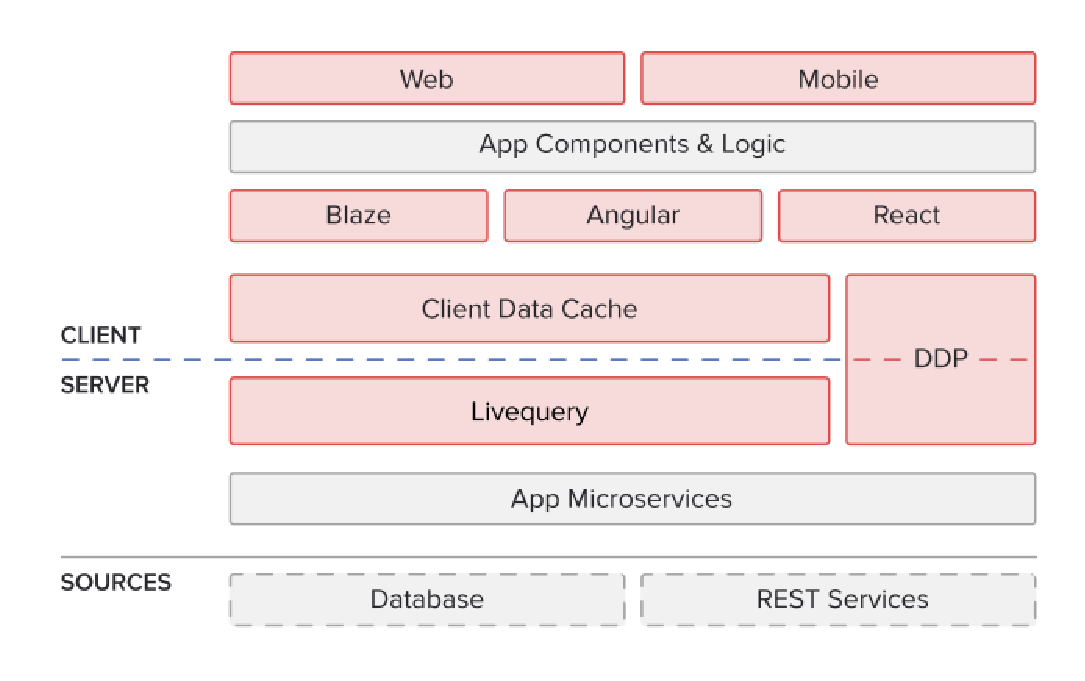
\includegraphics[width=.9\linewidth]{figuras/meteor-arq.eps}
  	\caption{Representação da arquitetura cliente-servidor do \textit{Meteor}.}
	\small{Fonte: \cite{meteor2015}}
  	\label{fig:meteor-arq}
\end{figure} 

Além dos motivos citados anteriormente, outro motivo para adoção desta plataforma como objeto de estudo foi a identificação das seguintes fraquezas: o componente de reprodução de vídeo não suporta conteúdo hipermidiático, o que pode ser visto na figura \ref{fig:hyp_reprod}; também a tela de construção de subvídeos, que possibilita a criação da interatividade do conteúdo, não favorece o autor do curso no sentido de apresentar apenas a estrutura de decisão ao final de cada vídeo, mostrado na figura \ref{fig:hyp_constr}.

\begin{figure}[h!]
	\centering
  	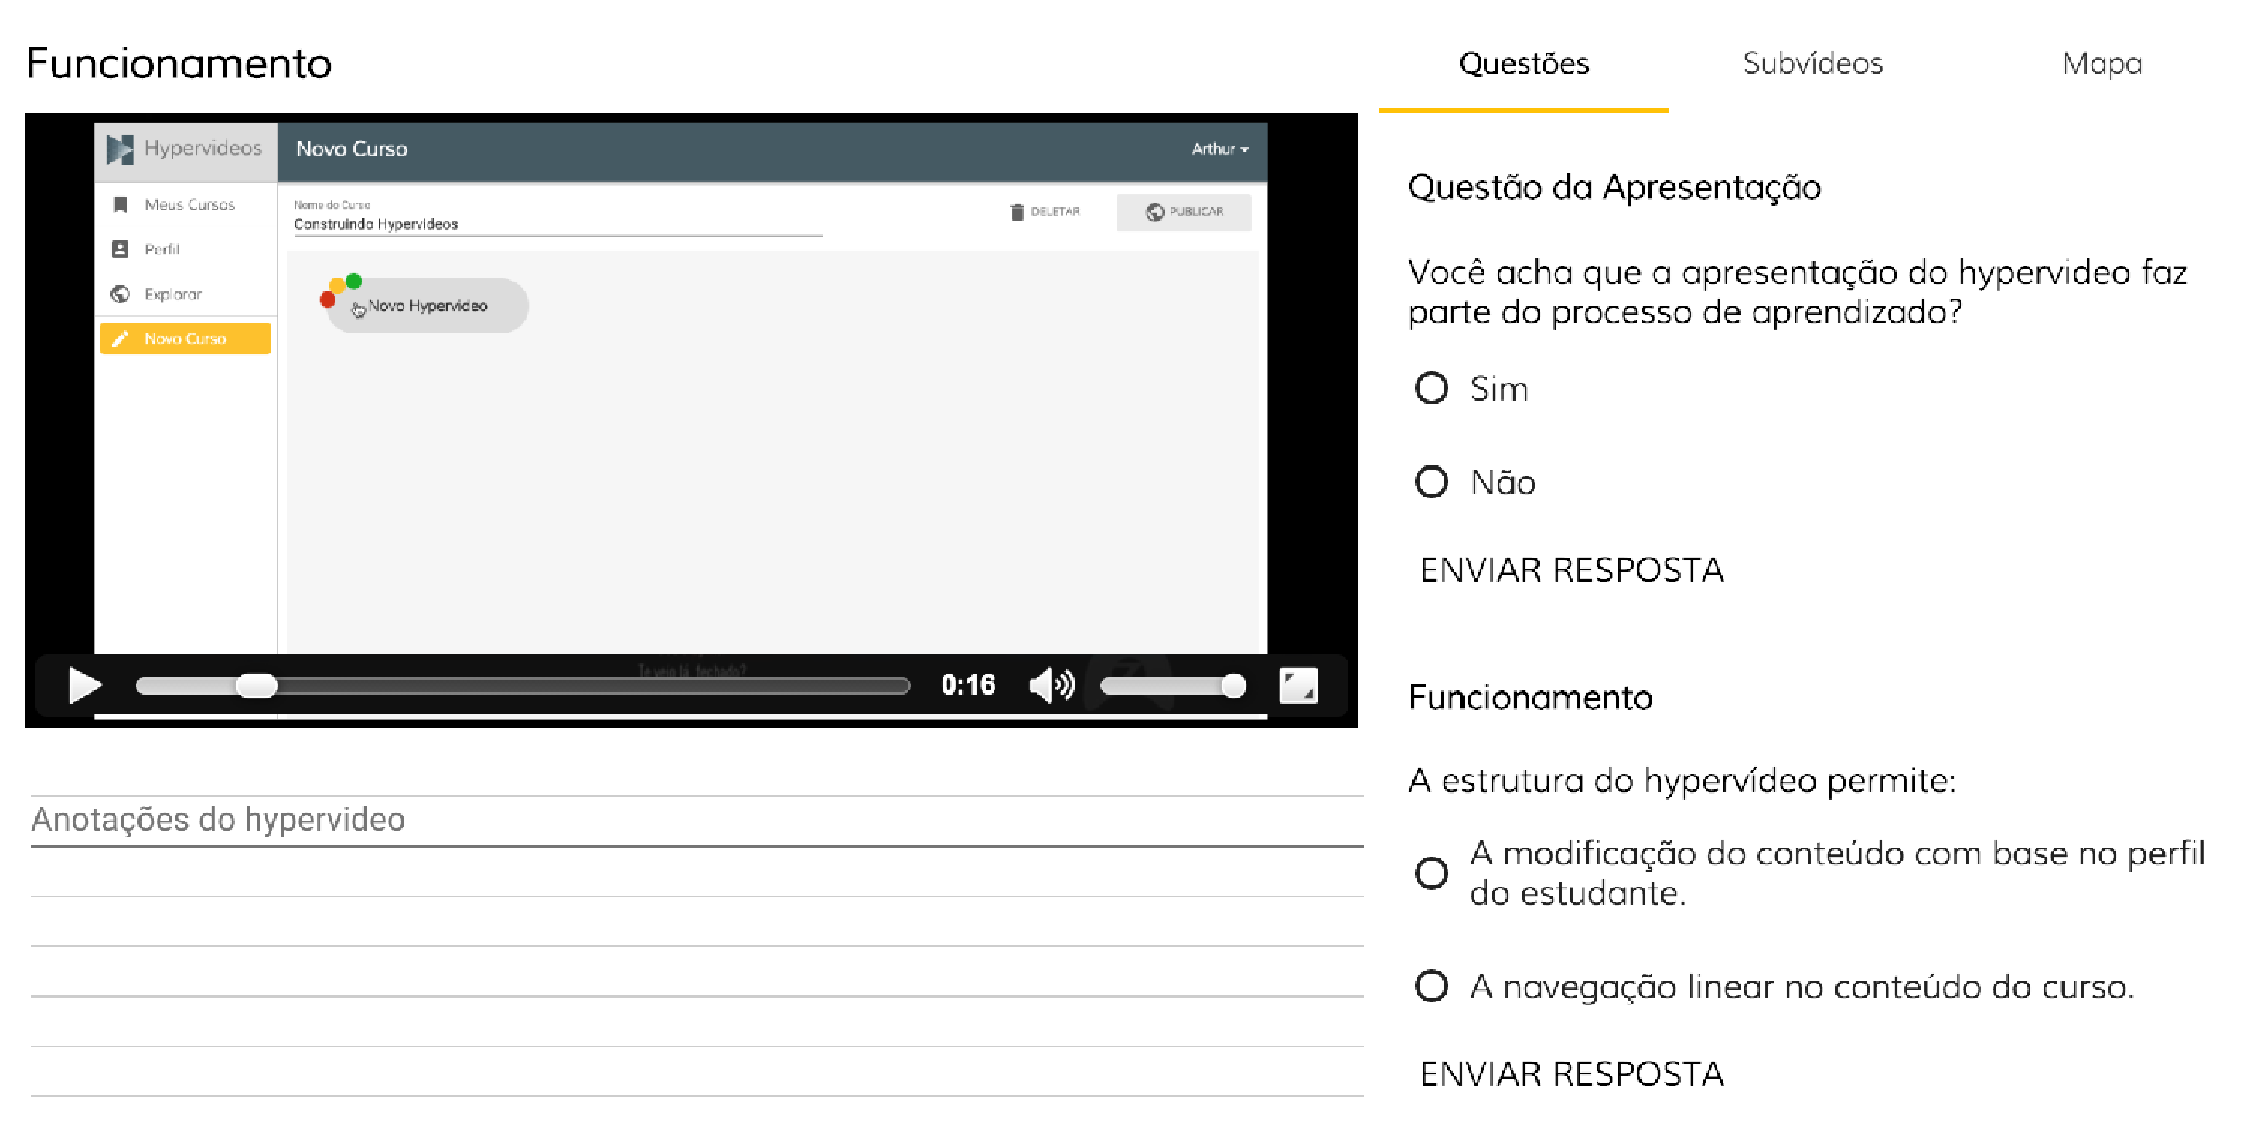
\includegraphics[width=.9\linewidth]{figuras/reproducao_hyp.eps}
  	\caption{Tela de apresentação do hypervídeos.}
	\small{Fonte: \cite{arthurtcc}}
  	\label{fig:hyp_reprod}
\end{figure} 

\begin{figure}[h!]
	\centering
  	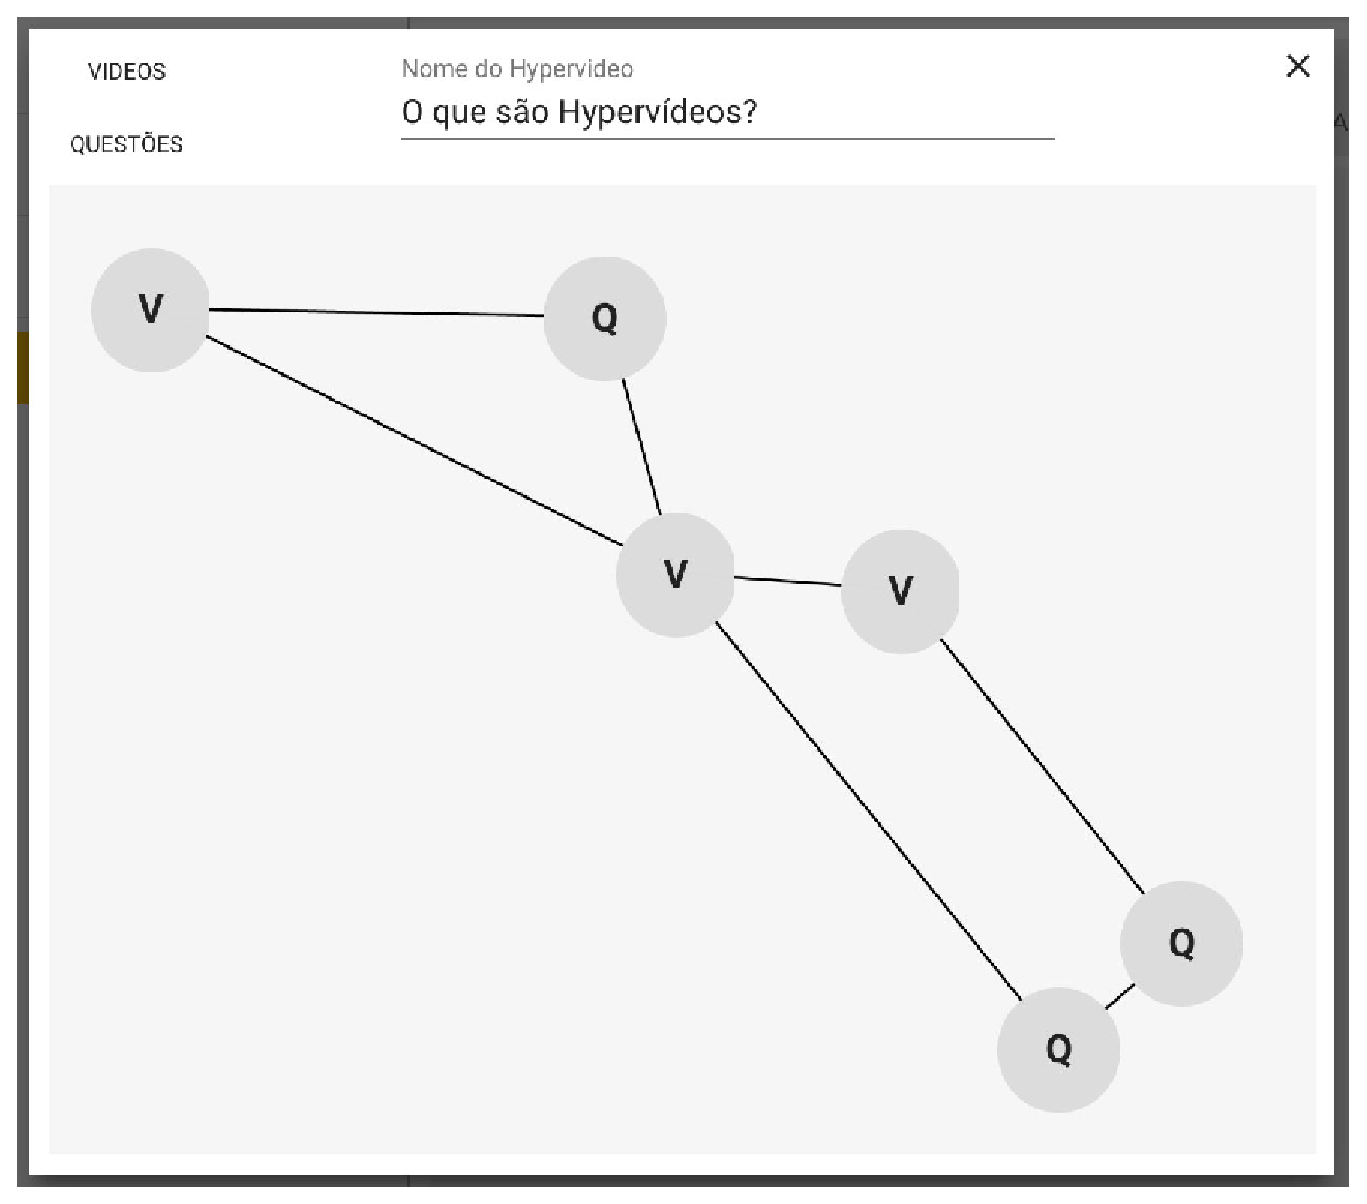
\includegraphics[width=.7\linewidth]{figuras/construcao_hyp.eps}
  	\caption{Tela de construção de material do hypervídeos.}
	\small{Fonte: \cite{arthurtcc}}
  	\label{fig:hyp_constr}
\end{figure} 

\section{Módulo de Criação de Anotações}

O módulo de criação de anotações tem como principais objetivos facilitar a criação e análise das anotações. Para compreender como este módulo funciona e como foi estruturado é necessário entender os passos envolvidos desde a visão do componente até a persistência dos dados.

O Componente de hípervideo segue o padrão arquitetural MVC, logo a visão do módulo de criação possui responsabilidades relacionadas apenas à eventos e aspectos visuais. Visualmente o componente de criação de anotações é semelhante ao componente de reprodução, mas com algumas diferenças sutis. O componente possui um reprodutor de vídeo com controles assim como o componente de visualização de hipervídeos, o intuito é permitir que o professor autor, criar as anotações e conferir o quanto antes o resultado gerado realizada, além de facilitar a identificação de qual momento deve ser adicionada a anotação.

Diferentemente do componente de visualização de hipervídeos, o módulo de criação de anotações se comporta exibindo um \textit{menu} de opções de tipos de anotações na parte superior do componente ao detecta um clique de seleção, observe na figura \ref{fig:hp_closed_tab}. Na atual configuração do sistema, a anotação pode ser um subvídeo ou questões. Ao selecionar o tipo de anotação que se deseja adicionar, é necessário inserir as mídias e em seguida as informações da anotação, sendo estas diferentes para cada tipo diferentes de anotação. Na figura \ref{fig:hp_open_tab} é apresentada a tela em que o usuário pode carregar vídeos para criar anotações, já na figura \ref{fig:hp_editing} é apresentada a tela onde o usuário deve inserir os dados da anotação.

\begin{figure}[h!]
	\centering
	\begin{subfigure}{.45\textwidth}
	  	\centering
  		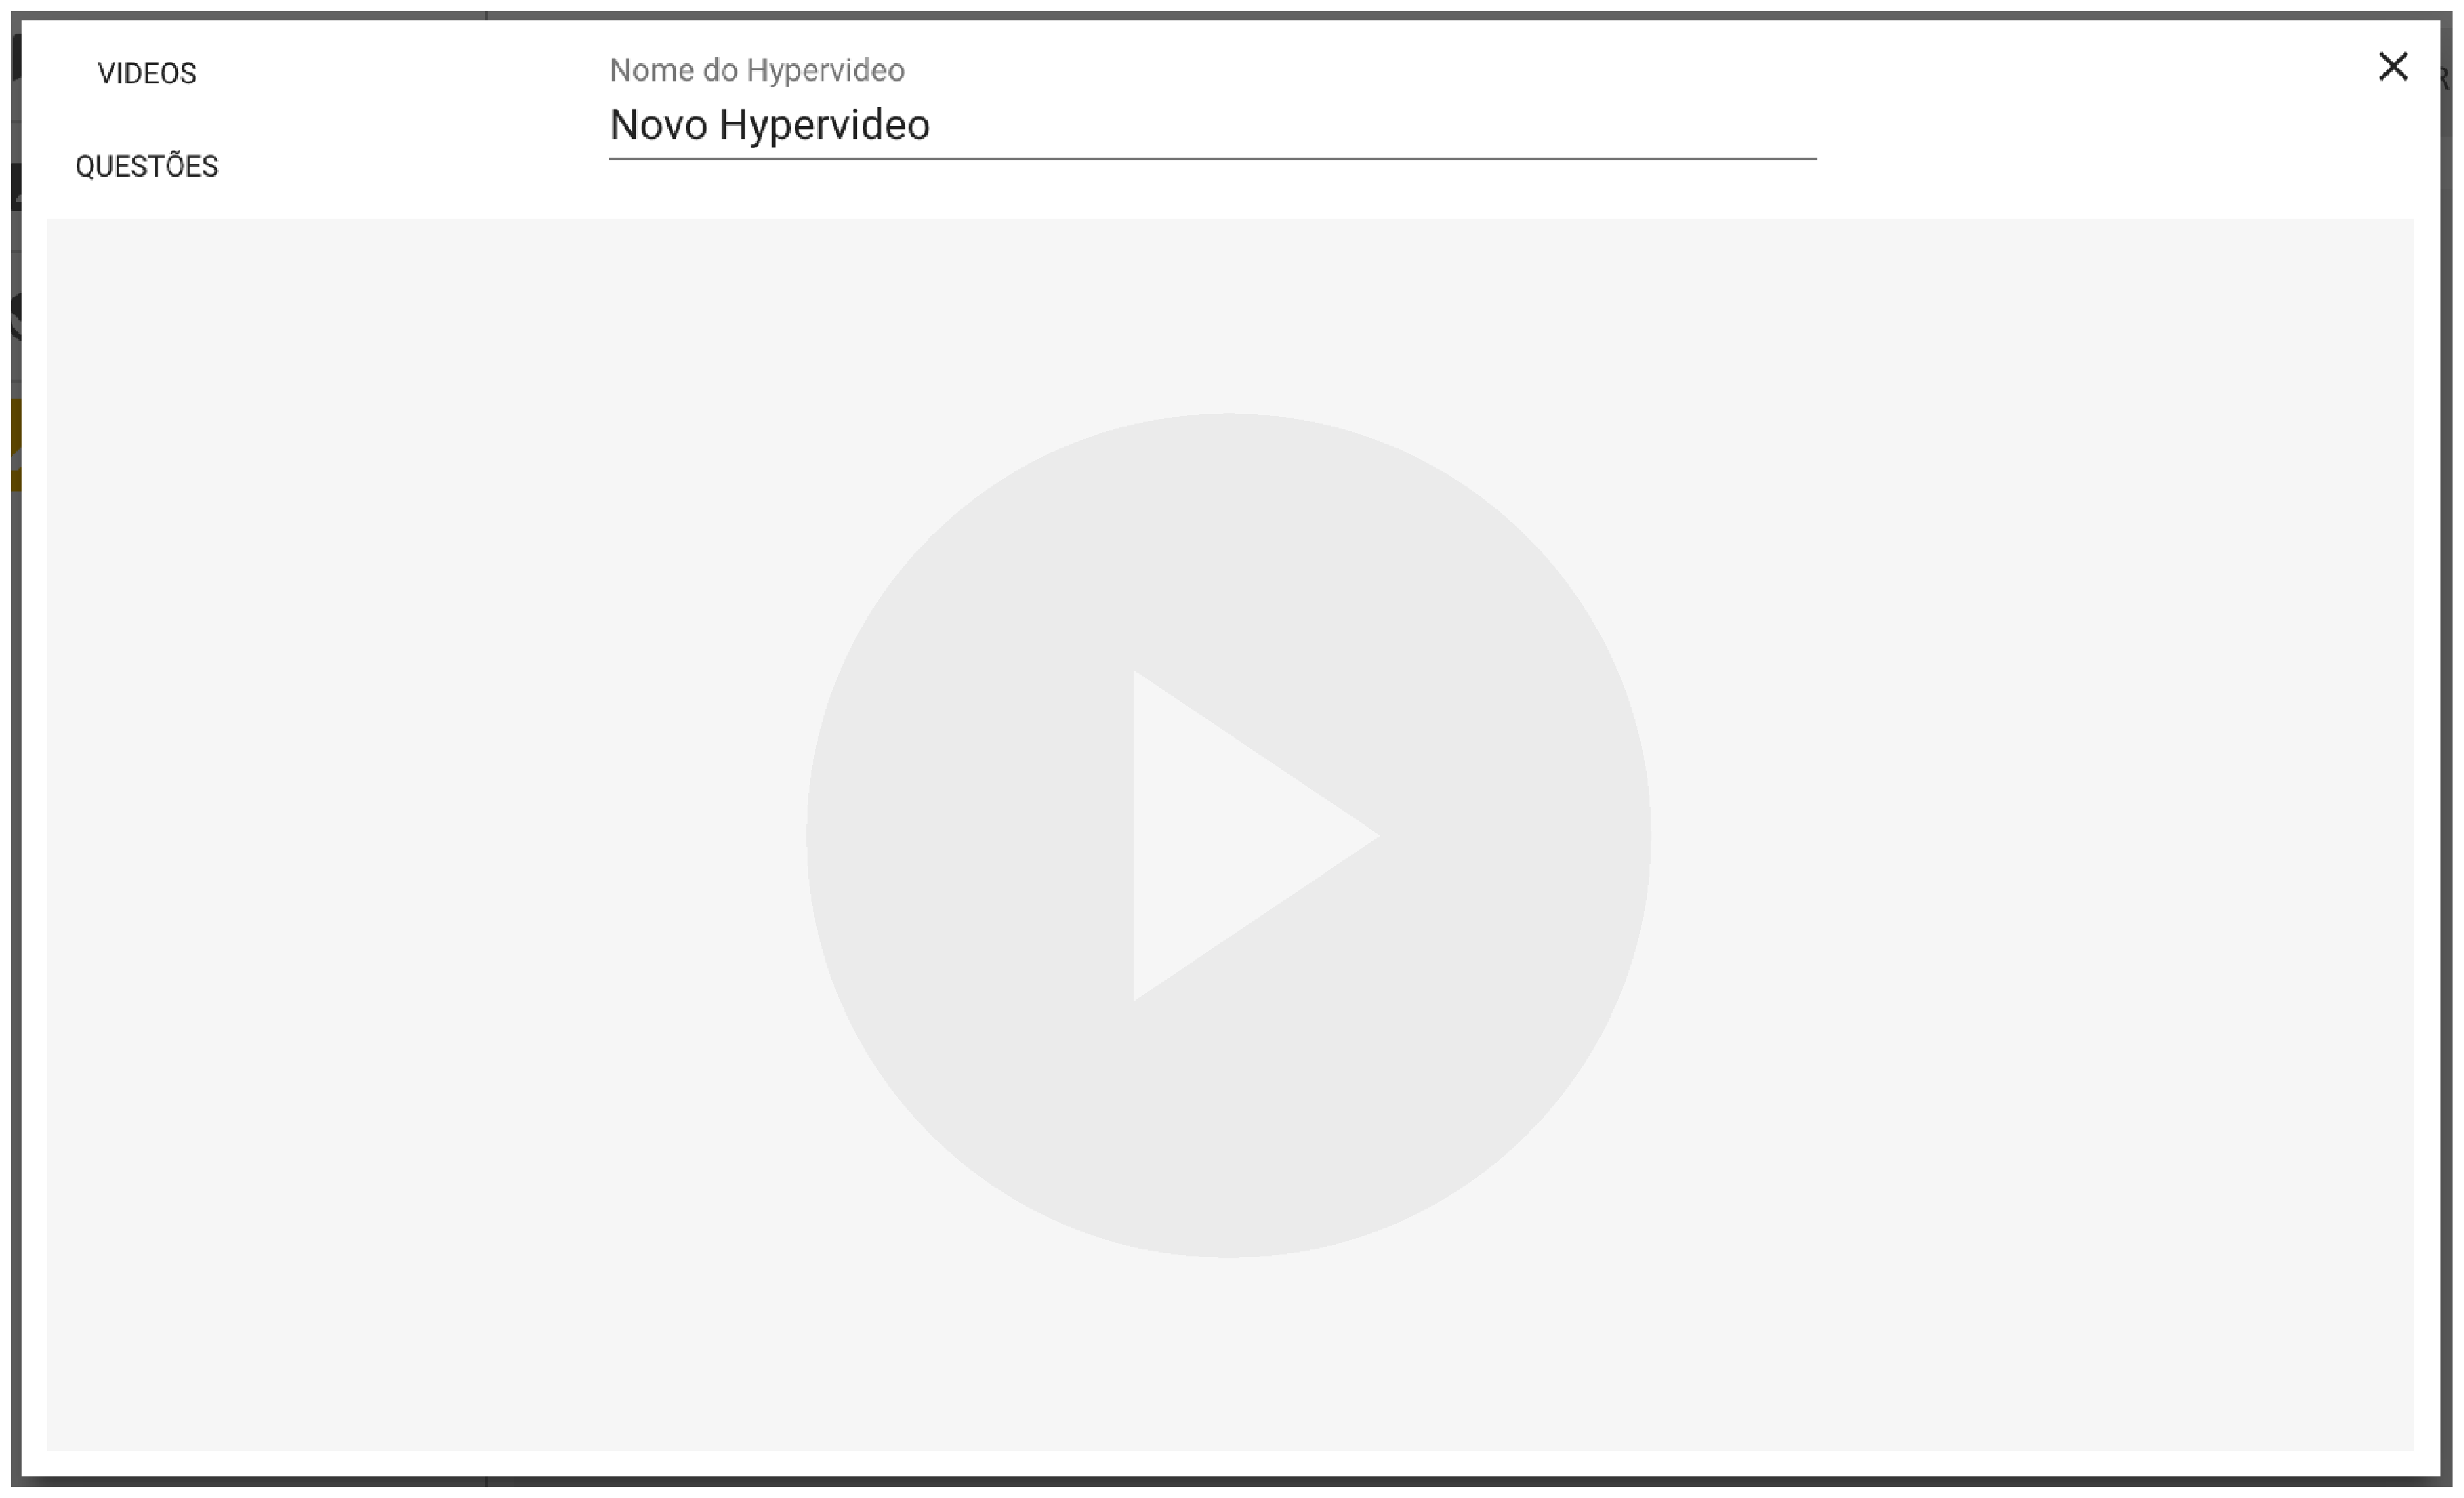
\includegraphics[width=.9\linewidth]{figuras/composer_tab_closed.eps}
  		\caption{Componente vazio.}
		\small{Fonte: Próprio}
	  	\label{fig:hp_closed_tab}
  	\end{subfigure}%
	\begin{subfigure}{.45\textwidth}
	  	\centering
  		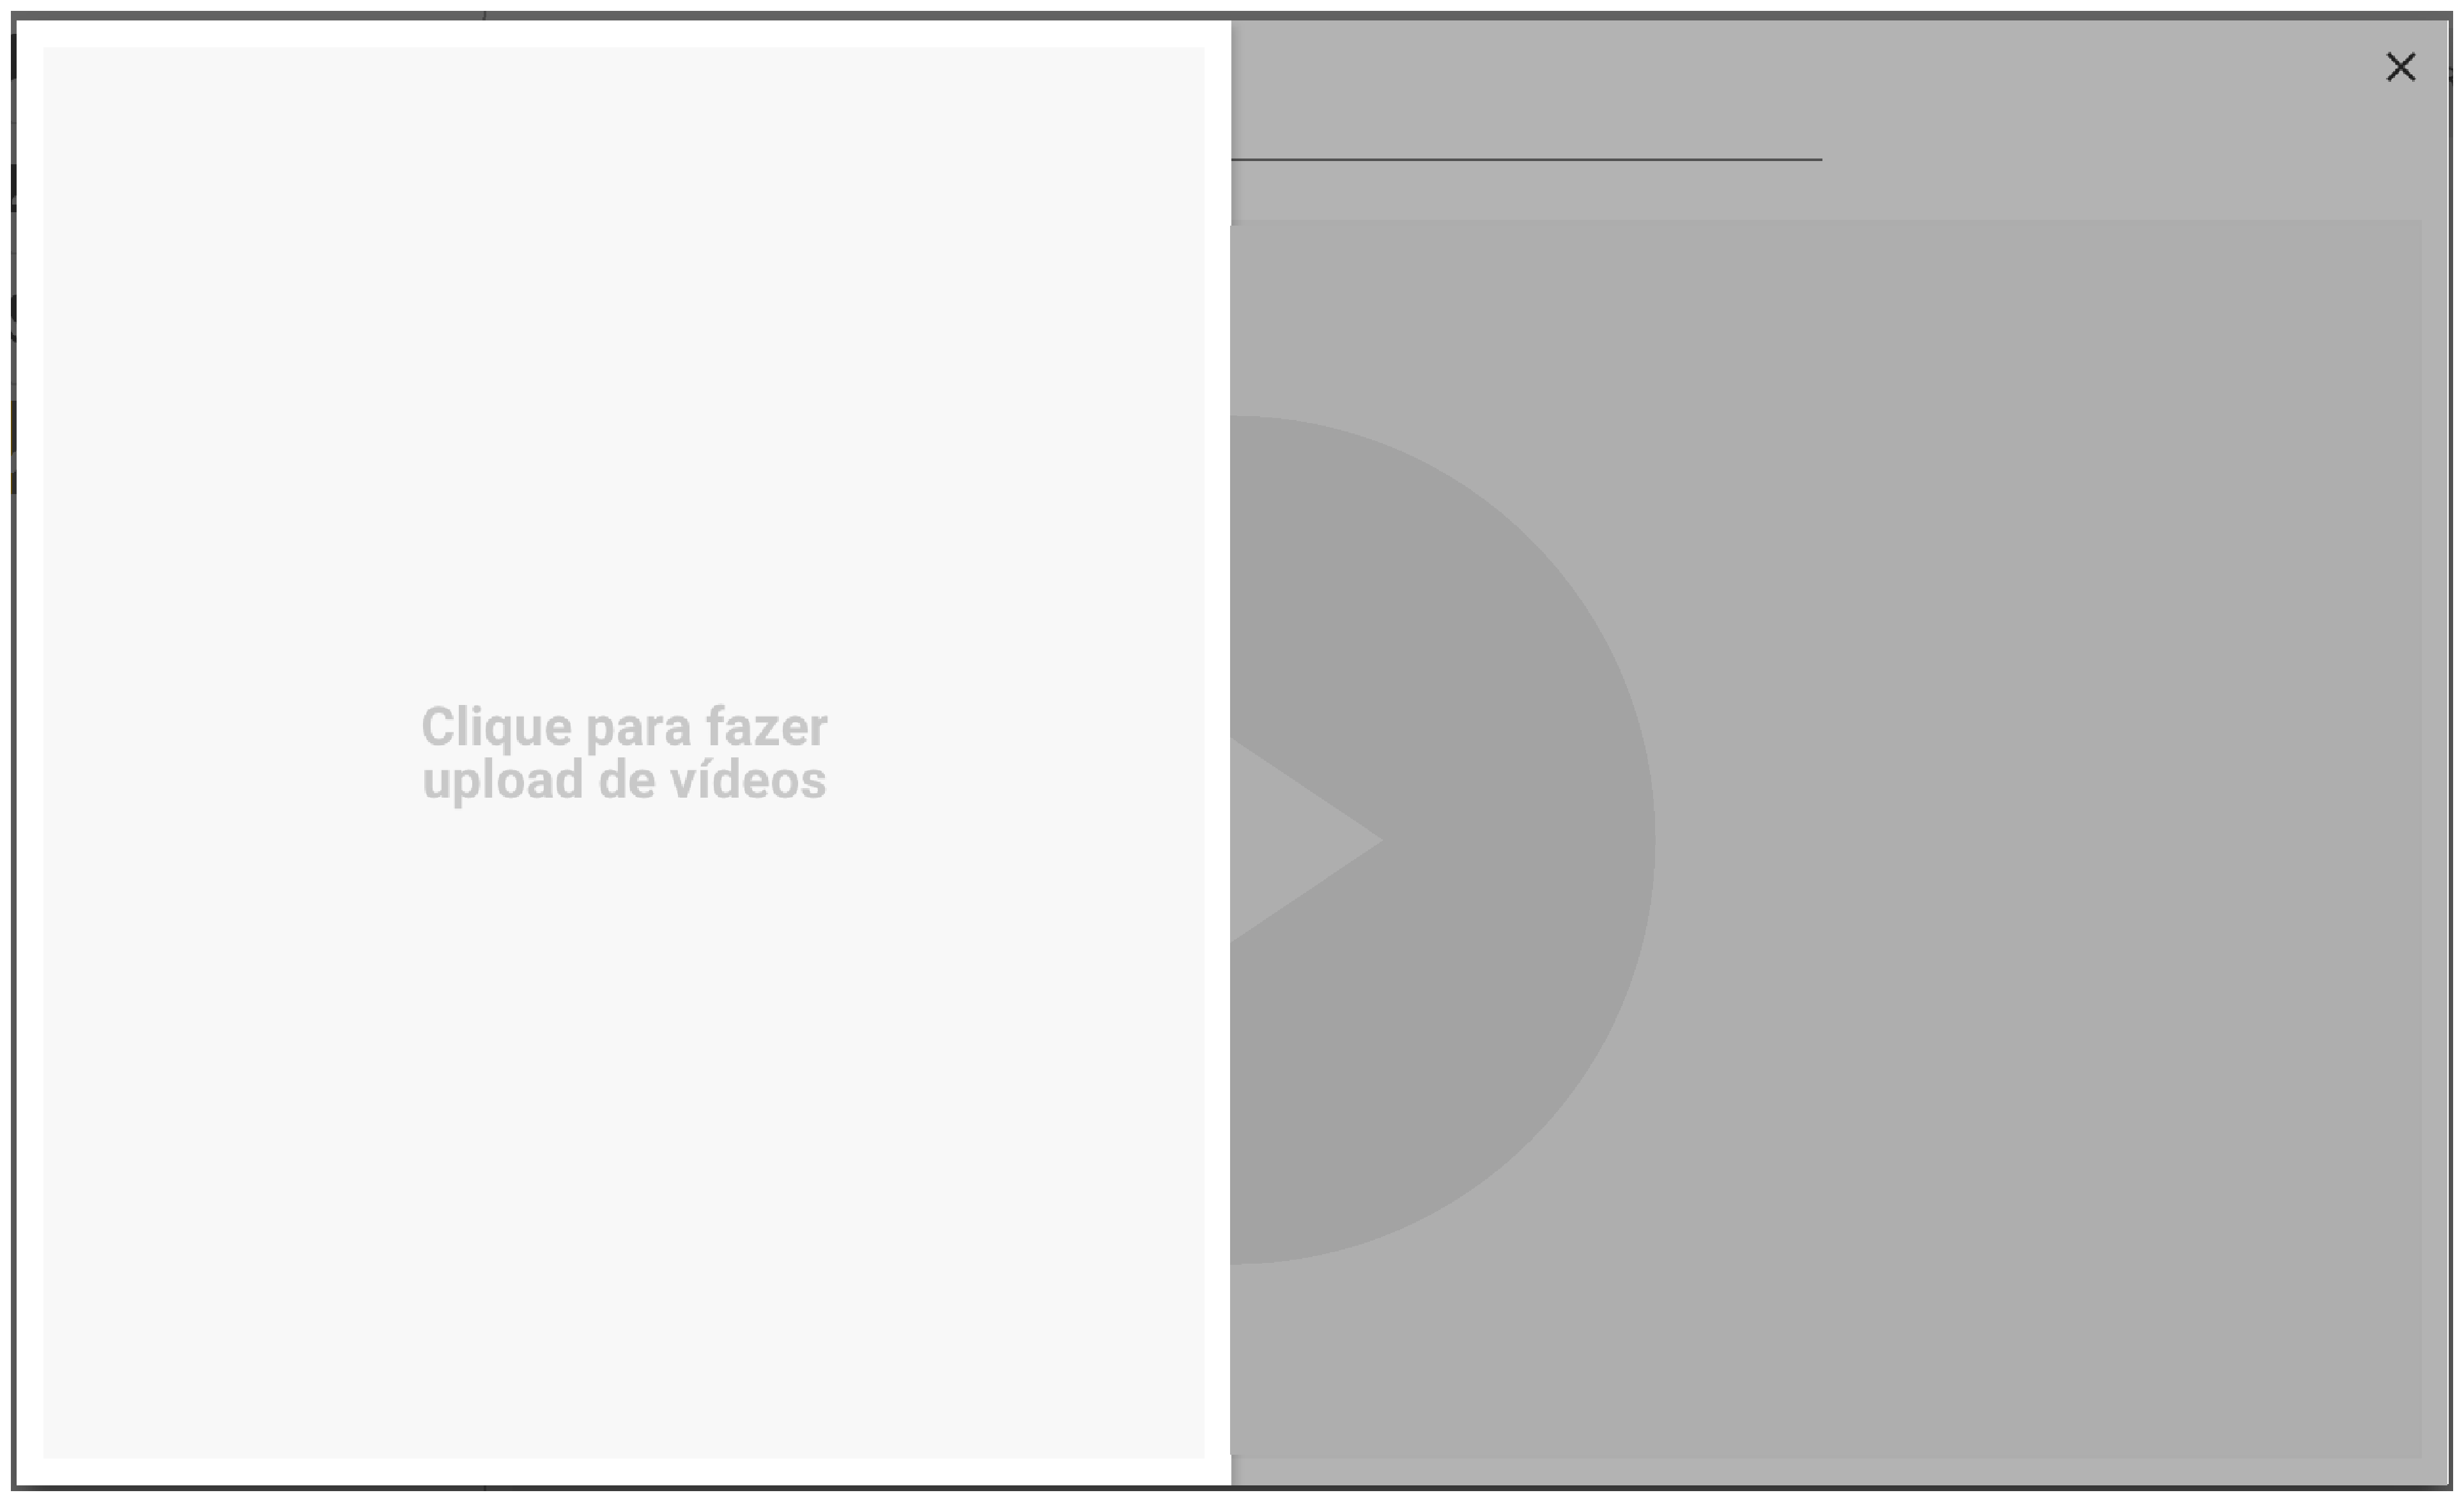
\includegraphics[width=.9\linewidth]{figuras/composer_tab_opened.eps}
  		\caption{Aba para adição de vídeos.}
		\small{Fonte: Próprio}
	  	\label{fig:hp_open_tab}
  	\end{subfigure}%
	\caption{Componente de construção de hipervídeo.}
\end{figure} 

\begin{figure}[h!]
	\centering
  	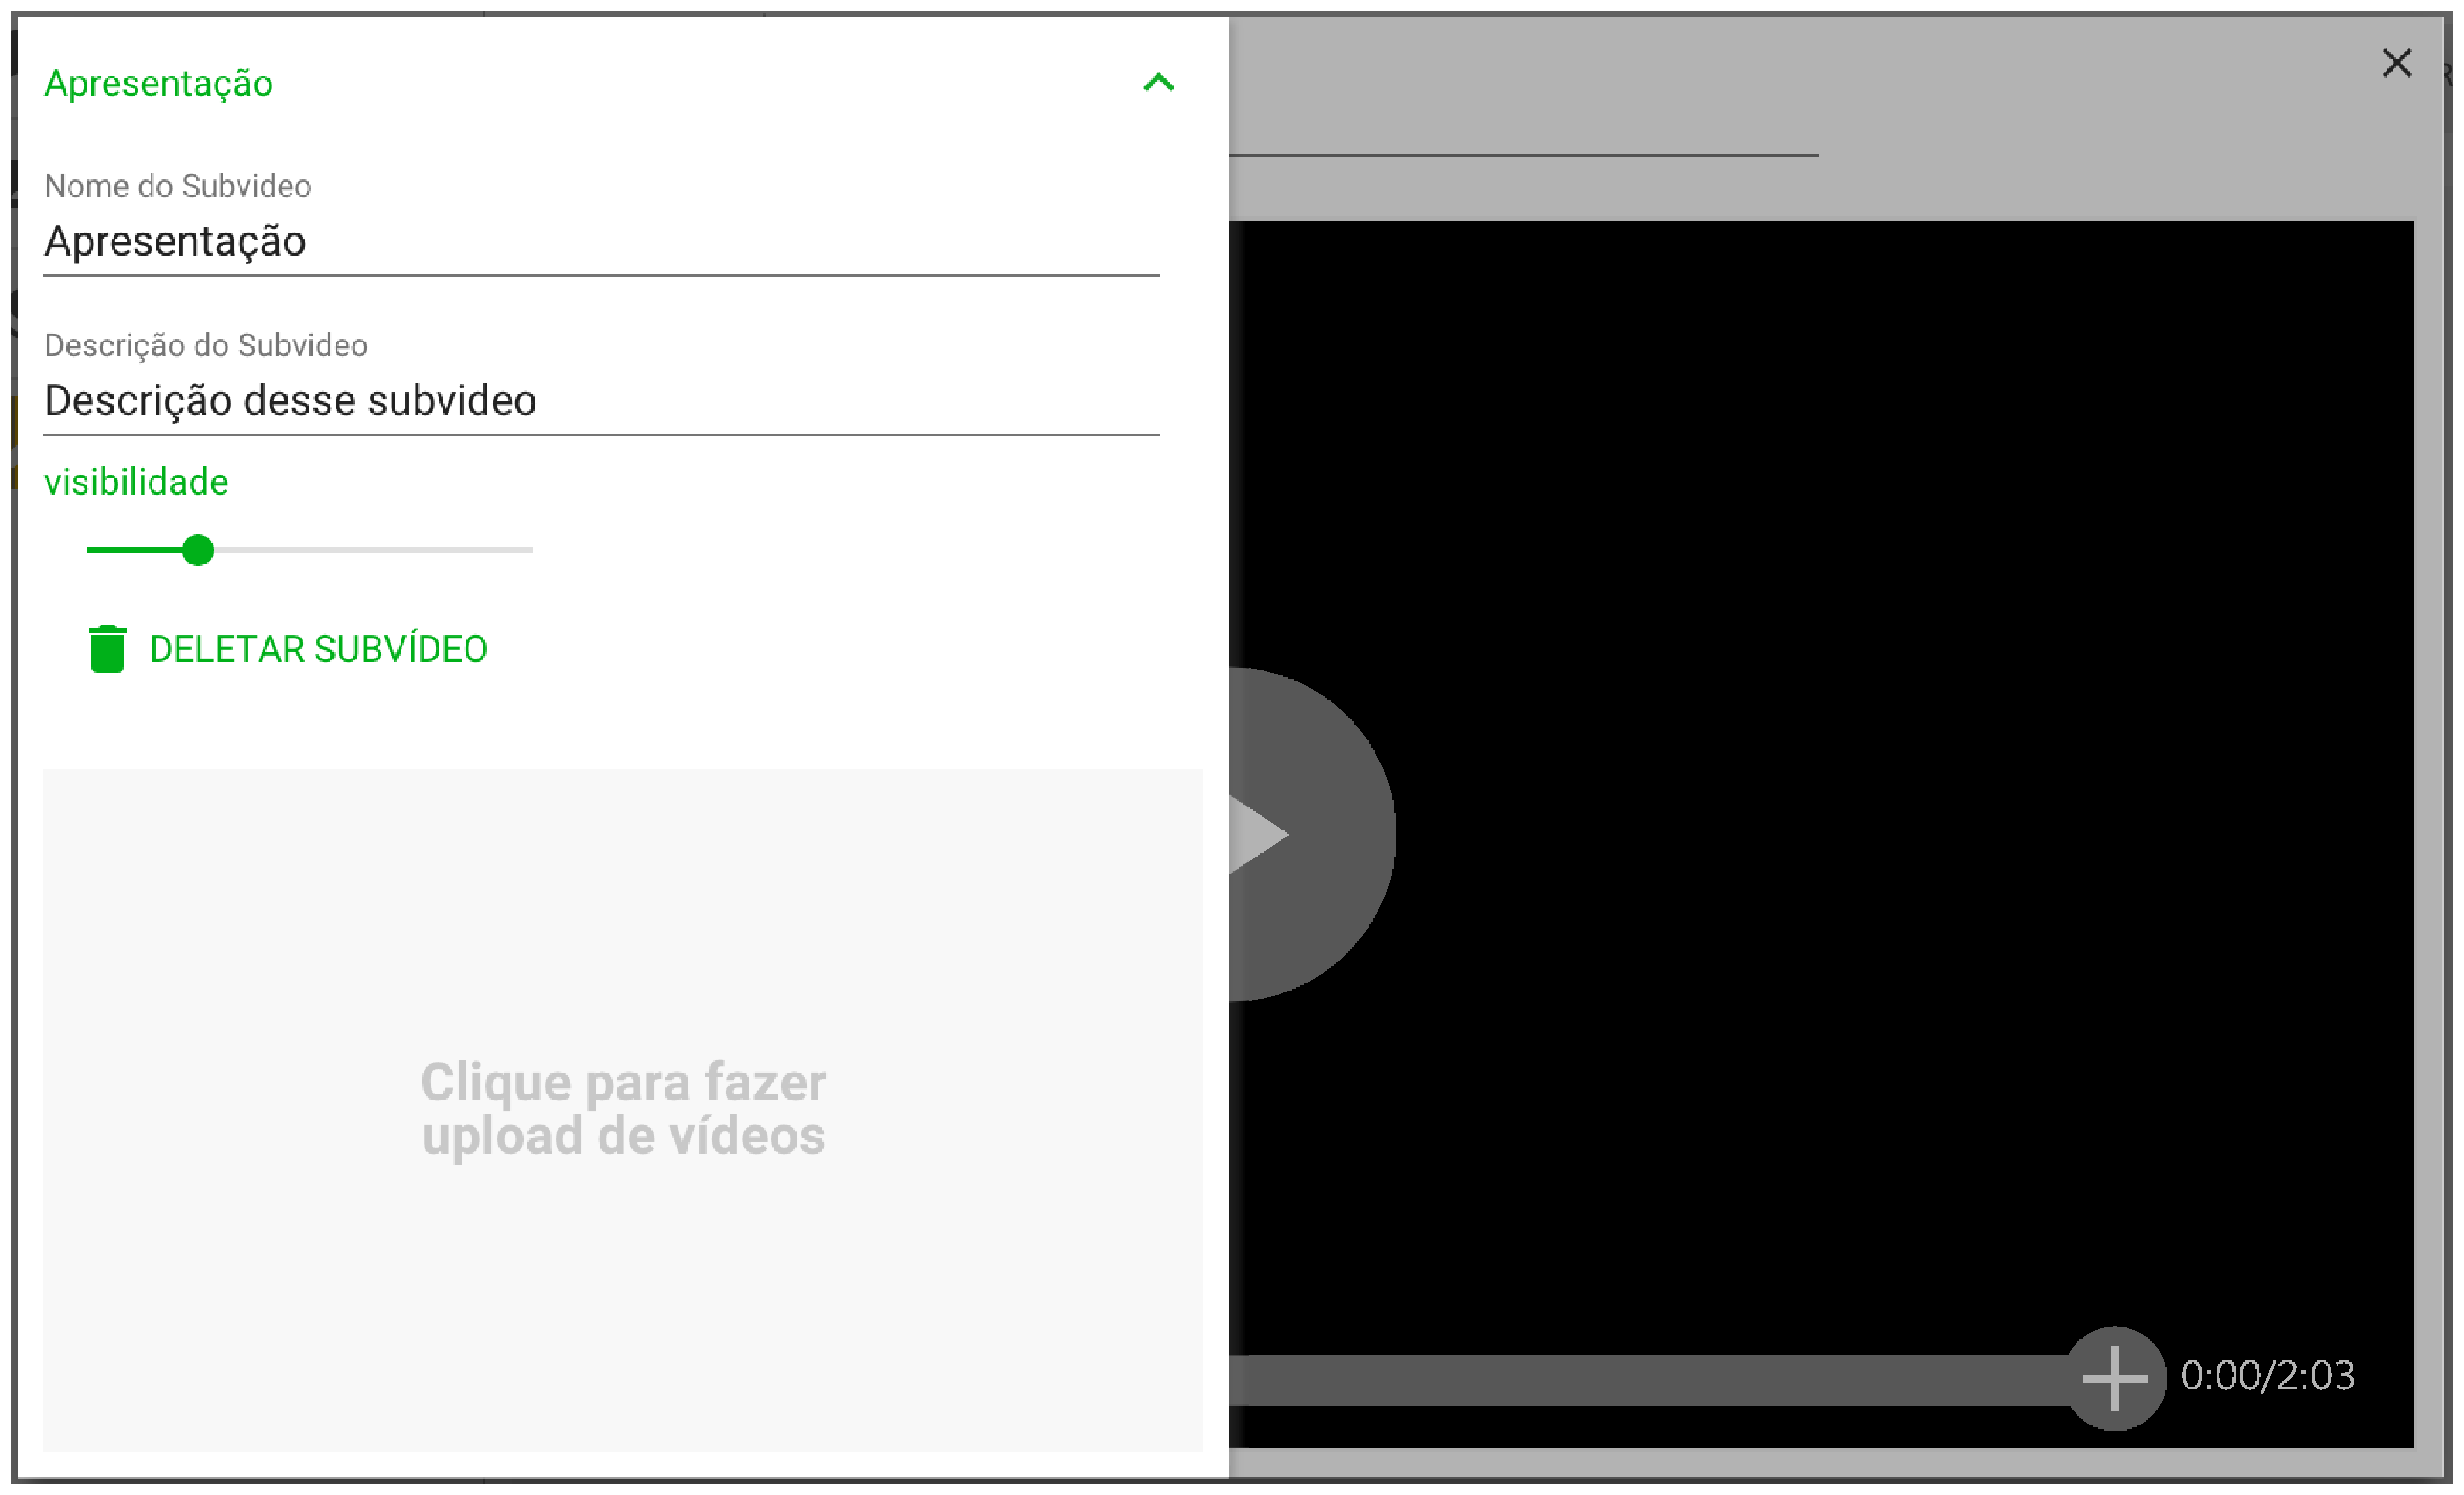
\includegraphics[width=.9\linewidth]{figuras/composer_video_added.eps}
  	\caption{Componente mostrando a tela de edição ativa de anotações.}
	\small{Fonte: Próprio}
  	\label{fig:hp_editing}
\end{figure} 

Ao criar uma anotação que referencia um subvídeo deve ser informado qual a mídia audiovisual que será utilizada, em qual tempo deve iniciar a reprodução e qual a duração da anotação. Já para adicionar anotações do tipo questões deve ser informado o enunciado da questão, as alternativas e em qual tempo as questões devem ser exibidas. Neste momento é perceptível que o atributo de tempo inicial é intrínseco a todas as anotações.

De modo a não quebrar a arquitetura MVC, as informações inseridas são encaminhadas para a camada de controle através de disparo de eventos e da mesma forma repassadas para o modelo para que os dados possam então serem validados e gravados na base de dados em formato \textit{JSON}. Nesse momento é importante ressaltar que as anotações se tornarão uma camada adicional sobreposta aos vídeos quando utilizados pelo módulo de visualização.

Como as informações relevantes da anotação são exibidas em tela, é possível analisar se os dados inseridos estão corretos, e também possibilita que outras anotações já existentes possam ser acessadas para que sejam reaproveitadas, evitando que haja um trabalho repetido desnecessariamente.

A visão do componente está baseada na biblioteca \textit{Polymer}, o que permite muita flexibilidade com relação a reutilização do componente em outros sistemas e também com relação a criação de novos tipos de anotações, requerendo um conhecimento técnico consideravelmente menor e buscando a aderência à padrões \textit{web}. As ações dos componentes são implementadas utilizando a linguagem \textit{Javascript}, a mesma linguagem utilizada pelo \textit{Meteor} que é a base da plataforma Hypervídeos.

Ao utilizar o modo de reprodução o motor do módulo de reprodução é acionado, porém o funcionamento será abordado na seção seguinte.

\section{Módulo de Visualização de Hipervídeos}

Como foi mencionado, o módulo de visualização de hipervídeos funciona de modo ligeiramente diferente, seguiremos a mesma abordagem da seção anterior para entender o funcionamento.

Ao iniciar uma reprodução de hipervídeo, o módulo de visualização dispara um evento capturado pelo controle para requisitar que o modelo de dados recupere as informações das anotações gravadas na base de dados que contém o identificador do hipervídeo. Após conseguir estas informações o modelo de dados dispara um evento para encaminha-las para o controle que então inicia a reprodução do hipervídeo. No instante em que uma anotação deve ser apresentada o controle usa os atributos da anotação para buscar as mídias necessárias, em seguida empacota essas informações e envia para a visão novamente através de um disparo de evento notificando que o componente \textit{Polymer} referente ao tipo de anotação que deve ser exibido com os dados relevantes da anotação.

Quando exibida a visão da anotação, fica a cargo da visão lidar com a interação entre o usuário e o componente. É importante lembrar que a anotação não necessita de uma visão de forma compulsória, um exemplo disso é quando a anotação referencia um outro vídeo que deve substituir a mídia atual. No caso do componente de questões é possível que a anotação requeira que o vídeo em reprodução seja pausado e a tela escurecida, como um exemplo da aplicação das heurísticas de aprendizagem multimídia.

\section{Integração com a plataforma Hypervídeos}

A integração com a plataforma deve acontecer de modo a não ferir os princípios do MVC. Para realizar tal tarefa foi proposto o modelo de aquitetura que pode ser visto na figura \ref{fig:arquitetura_final}. Pode-se perceber que os elementos da arquitetura do componente se conectam com a plataforma em cada camada. 

\begin{figure}[h!]
	\centering
  	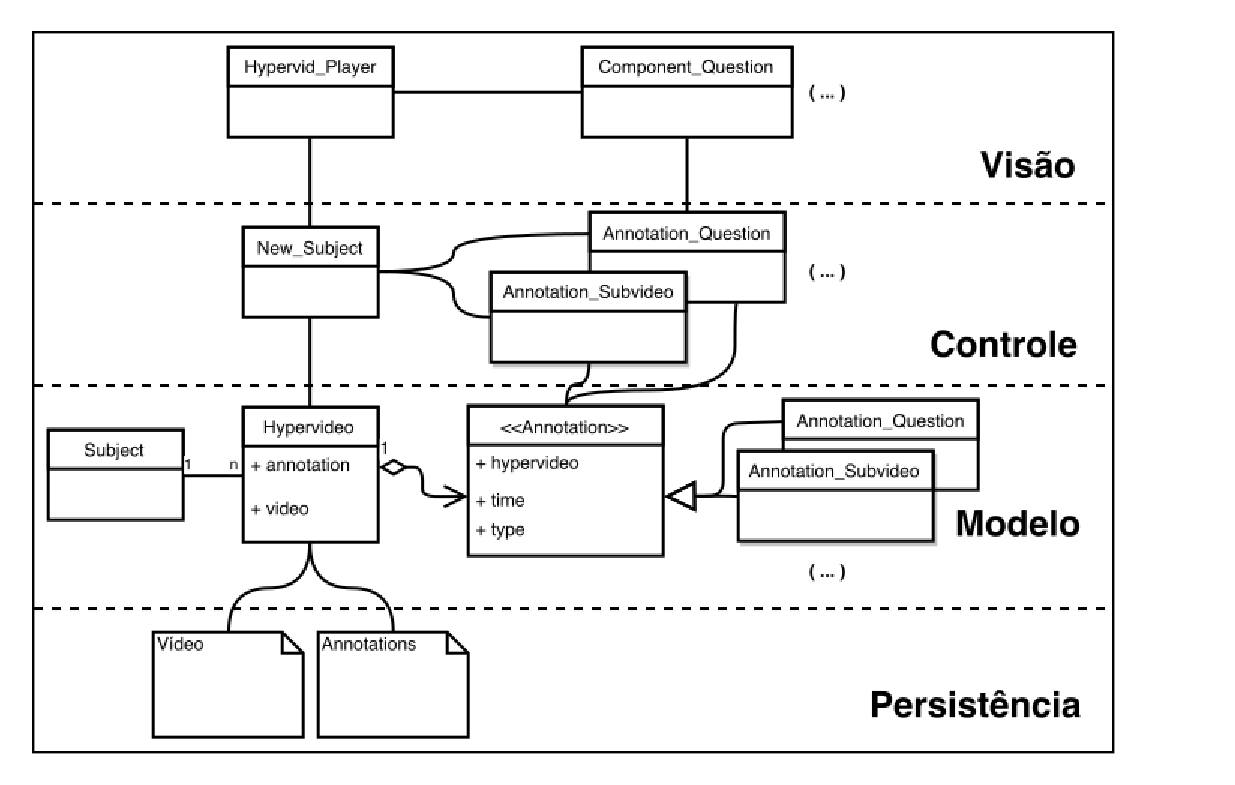
\includegraphics[width=.7\linewidth]{figuras/arquitetura.eps}
  	\caption{Arquitetura planejada para integração com Hypervídeos.}
	\small{Fonte: Própria.}
  	\label{fig:arquitetura_final}
\end{figure}

Porém para elaboração deste trabalho foi proposto uma prova de conceito para que se verificasse a possibilidade real de construção do componente. Esta prova de conceito segue uma arquitetura similar, porém mais simples que a que se pretende construir no produto final, esta arquitetura pode ser analisada na figura \ref{fig:arquitetura_probe}. 

\begin{figure}[h!]
	\centering
  	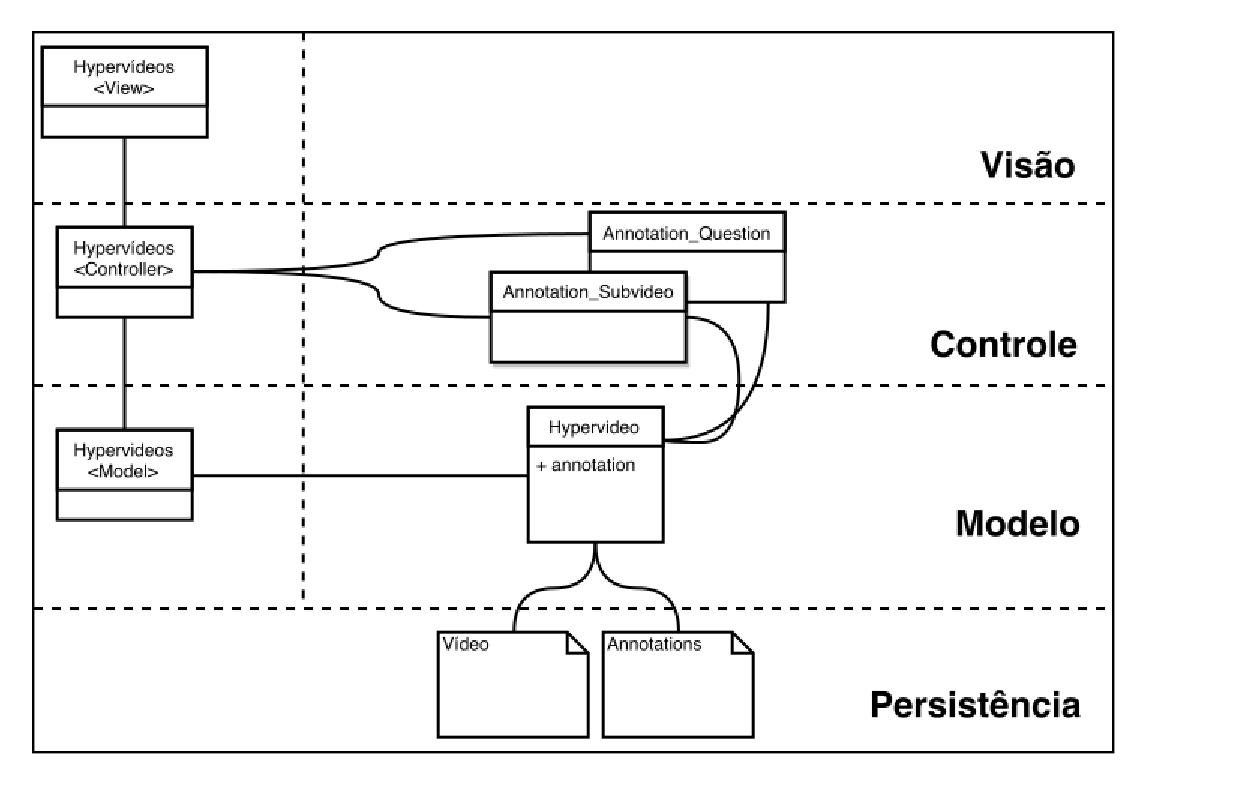
\includegraphics[width=.7\linewidth]{figuras/arquitetura_simpler.eps}
  	\caption{Arquitetura da prova de conceito realizada.}
	\small{Fonte: Própria.}
  	\label{fig:arquitetura_probe}
\end{figure}

Esta arquitetura se mostrou eficaz aos objetivos propostos, permitindo a integração com a plataforma, criação de anotações, e visualização do vídeo em conjunto com conteúdo anotado de forma sobreposta. Esta arquitetura não beneficia a expansão dos componentes de anotação, porém é suficiente para inferir que é possível adicionar esta característica por meio de refatorações no código. 